\documentclass[12pt,a4paper]{article}

\usepackage[T1]{fontenc}
\usepackage[utf8]{inputenc}
\usepackage[english]{babel}
\usepackage{geometry}
\geometry{top=2.5cm, bottom=2.5cm, left=2.5cm, right=2.5cm}
\usepackage{graphicx}
\usepackage{float}
\usepackage{subcaption}
\usepackage{booktabs}
\usepackage{tabularx}
\usepackage{listings}
\usepackage{xcolor}
\usepackage{hyperref}
\hypersetup{colorlinks=true, linkcolor=blue, citecolor=blue, urlcolor=blue}
\usepackage{setspace}
\usepackage{parskip}
\usepackage{microtype}
\usepackage{enumitem}
\usepackage{amsmath}
\usepackage{fancyhdr}
\pagestyle{fancy}
\fancyhf{}
\rhead{\small IRIS 2026 Hackathon}
\lhead{\small Br\"{u}ne, Corazza, Longo, Sapienza, Vagnoni}
\cfoot{\thepage}
\renewcommand{\headrulewidth}{0.4pt}

\onehalfspacing
\setlength{\parindent}{0pt}

\lstdefinelanguage{Turtle}{
  morekeywords={a,xsd,ex,legal,ipronto},
  morestring=[b]{"},
  morecomment=[l]{\#},
  sensitive=false,
}
\lstset{
  basicstyle=\footnotesize\ttfamily,
  keywordstyle=\color{blue!70!black}\bfseries,
  stringstyle=\color{brown},
  commentstyle=\color{gray}\itshape,
  breaklines=true,
  frame=single,
  framerule=0.4pt,
  rulecolor=\color{gray!40},
  backgroundcolor=\color{gray!5},
  aboveskip=6pt,
  belowskip=4pt,
}

% -----------------------------------------------------------------------
\title{
  \textbf{A Neuro-Symbolic System for Querying and Monitoring\\[0.3em]
  Copyright Compliance Across National Legislations}\\[0.6em]
  \large Authentic Source Attribution, Point-in-Time Navigation,\\[0.2em]
  and SPARQL-Based WIPO Compliance Checking over Akoma Ntoso
}

\author{
  John Frederic Br\"{u}ne \and
  Michele Corazza \and
  Generoso Longo \and
  Salvatore Sapienza \and
  Simone Vagnoni\\[0.4em]
  \small LAST-JD Programme, Universit\`{a} di Bologna, Italy\\[0.2em]
  \small Supervisor: Prof.\ Monica Palmirani
}

\date{May 2026}

% -----------------------------------------------------------------------
\begin{document}
\maketitle
\thispagestyle{fancy}

% ── Abstract ────────────────────────────────────────────────────────────
\begin{abstract}
\noindent
We present a neuro-symbolic web application for querying intellectual
property (IP) law across nine national jurisdictions and verifying their
compliance with WIPO treaty obligations. The system combines a large
language model (LLM) for multilingual query enrichment and answer
generation with a symbolic pipeline built on an RDF Knowledge Graph (KG)
structured over the IPROnto ontology, SPARQL-based retrieval, and Akoma
Ntoso (AKN) XML legal documents. Two architectural contributions are
central: \textbf{(i) authentic source attribution}, which surfaces FRBR
Work URIs and ELI identifiers extracted from each AKN corpus, linking
every answer to its official legislative source; and \textbf{(ii)
point-in-time navigation}, which resolves any of the 68 historical AKN
expressions of the Italian \emph{Legge} 633/1941 (1941--2025) in force at
a user-specified date. A pure symbolic compliance checker, grounded in
integer-typed RDF triples and \texttt{ipronto:compliesWith} links, compares
national copyright duration against the Berne Convention Art.~7 minimum
without any LLM involvement, achieving sub-20\,ms latency. Empirical
verification across all nine jurisdictions confirms correct compliance
verdicts, accurate FRBR extraction, and day-level temporal precision.

\medskip
\noindent\textbf{Keywords:} Akoma Ntoso, FRBR, ELI, IPROnto, Knowledge
Graph, neuro-symbolic AI, point-in-time, SPARQL, WIPO Berne Convention,
copyright compliance
\end{abstract}

\newpage

% ── 1. Introduction ─────────────────────────────────────────────────────
\section{Introduction}

The law creates rights. Formal representations make them computable.

Monitoring the alignment between national legislation and international
intellectual property treaties is a labour-intensive task. To answer
``Is the Italian \emph{Legge}~633/1941 compliant with Article~7 of the
Berne Convention?'' a jurist must (1)~locate the relevant provision in the
national act, (2)~extract its normative value (e.g.,~70~years \emph{post
mortem auctoris}), and (3)~compare it semantically with the treaty minimum
(50~years pma). Repeating this across the nine jurisdictions covered by
WIPO requires machine-readable representations of legal norms.

Large Language Models (LLMs) offer fluent natural-language understanding
but lack grounding in authoritative legal sources and are prone to
hallucination~\cite{huang2023}. Symbolic Knowledge Graphs (KGs) encode
structured facts precisely but cannot handle multilingual query ambiguity.
A \textbf{neuro-symbolic} integration~\cite{hitzler2022}---LLM for
understanding, KG for retrieval and reasoning---is the appropriate
architecture for this task.

This paper presents an MVP developed during the IRIS 2026 Hackathon. Its
primary contributions are:
\begin{enumerate}[leftmargin=1.4em]
  \item A working end-to-end pipeline connecting multilingual LLM query
        enrichment to SPARQL retrieval over an AKN-grounded IPROnto KG.
  \item A pure symbolic compliance checker grounded in integer-typed RDF
        triples and \texttt{ipronto:compliesWith} links, requiring no LLM.
  \item \textbf{Authentic source attribution}: FRBR Work URIs and ELI
        identifiers extracted from AKN \texttt{FRBRWork} metadata, surfaced
        in the UI as verifiable hyperlinks to official legislative sources.
  \item \textbf{Point-in-time document navigation}: resolution of any of the
        68 historical AKN expressions of the Italian copyright act
        (1941--2025) in force at a user-specified date.
\end{enumerate}

% ── 2. Background ───────────────────────────────────────────────────────
\section{Background and Related Work}

\subsection{Akoma Ntoso and the FRBR/ELI Model}

Akoma Ntoso (AKN) is the OASIS standard for the XML representation of
legal and parliamentary documents~\cite{oasis2018,palmirani2011}. Its
hierarchical element tree (\texttt{<act>}, \texttt{<section>},
\texttt{<article>}, \texttt{<paragraph>}) assigns stable \texttt{eId}
attributes to every provision, enabling citation at the paragraph level
across time.

AKN embeds a FRBR metadata layer~\cite{ifla1998} encoding the
Work-Expression-Manifestation-Item hierarchy. The \texttt{<FRBRWork>}
element carries: \texttt{FRBRuri} (canonical Work-level URI);
\texttt{FRBRdate} (dated events typed by a \texttt{name} attribute, e.g.\
\emph{dateApplicability}, \emph{dateEntryInForce}); \texttt{FRBRalias}
(aliases, including the European Legislation Identifier,
ELI~\cite{eli2012}); and boolean flags \texttt{FRBRauthoritative} /
\texttt{FRBRprescriptive} marking official, legally binding sources.
These metadata fields are inconsistently populated across national
corpora---UK uses \texttt{FRBRprescriptive}, Switzerland uses
\texttt{FRBRauthoritative}, Germany omits both---a heterogeneity our
\texttt{akn\_metadata} module normalises with a priority fallback strategy.

\subsection{IPROnto}

IPROnto is an OWL ontology for the IP domain developed by the Distributed
Multimedia Applications Group (DMAG) at the Universitat Polit\`{e}cnica
de Catalunya~\cite{delgado2003}. It defines \texttt{ExploitationRight},
\texttt{ExceptionsRight}, and properties for jurisdiction, duration, and
rights grants. We use the IPROnto namespace as the backbone of our KG,
extending it with a \texttt{legal:} property vocabulary for SPARQL
querying.

\subsection{Neuro-Symbolic Legal AI}

LegalRuleML~\cite{palmirani2011lrml} formalises normative rules in XML,
supporting defeasibility and exceptions. Nardi et al.~\cite{nardi2026}
analyse IP ontologies in this volume. Our contribution is a complete,
runnable pipeline connecting LLM enrichment to SPARQL retrieval over
AKN-grounded RDF triples, extended with authentic source attribution and
temporal resolution.

% ── 3. Architecture ─────────────────────────────────────────────────────
\section{System Architecture}

\begin{figure}[H]
  \centering
  
\includegraphics[width=0.92\textwidth]{MVP_proposal_diagram.png}
  \caption{End-to-end pipeline. Shaded modules are neural (LLM); white
  modules are symbolic (SPARQL, AKN XML, FRBR). The right panel of the
  UI exposes the FRBR meta bar and the point-in-time date picker for
  Italian documents.}
  \label{fig:arch}
\end{figure}

The pipeline has six stages. Stages~1 and~6a are neural; stages~2--5
and~6b are fully symbolic (Figure~\ref{fig:arch}).

\subsection{Stage 1 --- Multilingual Query Enrichment (Neural)}

The user question (any language) is passed to Gemini~2.0~Flash via the
OpenRouter API with a structured system prompt. The LLM returns a JSON
object validated by Pydantic~v2 against a \texttt{SPARQLParams} schema:
\texttt{Jurisdiction} (one of 9 country names, ``WIPO'', or ``Unknown''),
\texttt{Legal\_Topic} (``copyright duration'', ``economic rights'', or
``personal-use exception''), \texttt{Time\_Frame} (year range or
``Current''), and \texttt{User\_Objective} (English rephrasing).
Italian input --- e.g.\ ``quando scade il diritto d'autore in Francia?''
--- is correctly mapped to Jurisdiction=France, Legal\_Topic=copyright
duration.

\subsection{Stage 2 --- KG Retrieval (Symbolic / SPARQL)}

The normalised parameters select one of three SPARQL SELECT templates
executed against an in-memory rdflib graph loaded lazily on first request
from a Turtle file. Listing~\ref{lst:turtle} shows representative triples.

\begin{lstlisting}[language=Turtle,label=lst:turtle,
  caption={Core KG triples for Swiss copyright duration (excerpt).}]
ex:CH_duration  a ipronto:ExploitationRight ;
    legal:jurisdiction     "CH" ;
    legal:durationLiterary "70 years pma" ;
    legal:durationYears    70 ;            # xsd:integer
    ipronto:triggeredBy    "death of author" ;
    legal:articleRef       "Art. 29 URG" ;
    legal:frbrWorkUri      "https://www.admin.ch/eli/cc/..." ;
    legal:pointInTime      "2022-01-01"^^xsd:date ;
    legal:isAuthoritative  true^^xsd:boolean ;
    legal:compliesWith     ex:WIPO_berne_art7 .

ex:WIPO_berne_art7  a ipronto:ExploitationRight ;
    legal:jurisdiction  "WIPO" ;
    legal:durationYears 50 ;    # Berne minimum
    legal:articleRef    "Art. 7 Berne Convention" .
\end{lstlisting}

The \texttt{legal:durationYears} integer literal enables numeric compliance
comparison without string parsing at query time. When the jurisdiction is
unknown the system falls back to a pre-populated Berne Convention evidence
record, disclosed to the user.

\subsection{Stage 3 --- AKN Passage Extraction (Symbolic)}

The article reference from the KG (e.g.,\ ``Art.~29 URG'') is resolved to
an AKN \texttt{eId} by the ArticleLocator module, which walks the parsed
XML tree matching \texttt{<num>} element text. The corresponding AKN
element is rendered as styled HTML with a highlighted supporting span.
Both \texttt{<article>} (Swiss, French, Italian) and \texttt{<section>}
(German, UK) provision types are handled. AKN files are accessed at query
time only; they are not ingested into the KG.

\subsection{Stage 4 --- Authentic Source Attribution (Symbolic)}
\label{sec:frbr}

Module \texttt{scripts/akn\_metadata.py} extracts FRBR/ELI metadata from
each AKN document, normalising across the divergent attribute naming
conventions present in the nine corpora. It returns:

\begin{itemize}[leftmargin=1.4em]
  \item \textbf{Work URI} (\texttt{frbr\_work\_uri}): the canonical
        Work-level identifier, rendered in the UI as an ``Official Source''
        hyperlink --- e.g.\
        \href{https://www.legislation.gov.uk/ukpga/1988/48}%
             {\texttt{legislation.gov.uk/ukpga/1988/48}} for the UK CDPA.
  \item \textbf{Applicability date} (\texttt{point\_in\_time}):
        \texttt{FRBRdate[@name=dateApplicability]} or, where absent, the
        entry-into-force date; displayed as a dated badge.
  \item \textbf{ELI URI} (\texttt{eli\_uri}): from
        \texttt{FRBRalias[@name="eli"]}, present for Italy
        (\texttt{urn:lex:it:stato:legge:\ldots}) and Switzerland.
  \item \textbf{Authenticity flag} (\texttt{is\_authoritative}):
        \texttt{true} when \texttt{FRBRauthoritative} or
        \texttt{FRBRprescriptive} carries \texttt{value="true"}.
\end{itemize}

These fields are stored as KG triples at build time
(\texttt{legal:frbrWorkUri}, \texttt{legal:pointInTime},
\texttt{legal:isAuthoritative}) and returned in every API response. The
document viewer renders them as coloured badges (green for authenticated
sources, blue for the applicability date) and a clickable
official-source link.

\subsection{Stage 5 --- Point-in-Time Navigation (Symbolic)}
\label{sec:pit}

Italy is the only jurisdiction for which multiple historical AKN
expressions are available: 68~files from the Normattiva repository cover
\emph{Legge}~633/1941 from the original 1941~text through amendments to
December~2025. Files follow the naming convention:
\begin{center}
  \small\texttt{1941-07-16\_041U0633\_VIGENZA\_\textbf{YYYY-MM-DD}\_V\textit{n}.xml}
\end{center}
where \texttt{VIGENZA\_YYYY-MM-DD} is the date from which the version
entered into force (\emph{vigenza}). Module \texttt{scripts/point\_in\_time.py}
builds a sorted index of (valid\_from, path) pairs lazily on first call and
returns the latest version~$v$ such that $\mathrm{valid\_from}(v) \leq
d_{\mathrm{target}}$. A \texttt{POST /api/document} endpoint exposes this
capability. In the UI, Italian document results display a date picker;
selecting a date re-fetches the historical version and updates all FRBR
badges accordingly.

\subsection{Stage 6 --- Answer Generation and Compliance Checker}

\textbf{Stage~6a (Neural).}
For Q\&A queries the KG evidence (passage, article reference, document
title, FRBR Work URI) is serialised and passed to the LLM with a
grounding-focused prompt constrained to 2--4 sentences citing the article.

\textbf{Stage~6b (Symbolic).}
The compliance checker reads \texttt{legal:durationYears} from both the
country KG node and \texttt{ex:WIPO\_berne\_art7}, computes the margin,
and emits a structured verdict rendered as a side-by-side comparison
card. No LLM is involved; latency is under 20\,ms.

% ── 4. Implementation ───────────────────────────────────────────────────
\section{Implementation}

The system is a Flask web application with two UI modes---Q\&A and
Compliance Check---accessible via tab switching. The right panel is a
shared document viewer rendering AKN HTML, the FRBR meta bar, and---for
Italian documents---the point-in-time date picker.

\begin{table}[H]
\centering
\caption{Technology stack.}
\label{tab:stack}
\begin{tabularx}{\textwidth}{lX}
\toprule
\textbf{Component} & \textbf{Technology} \\
\midrule
Web framework      & Flask (Python~3.12) \\
KG store           & rdflib~7 (in-memory, TTL serialisation) \\
XML parsing        & lxml \\
LLM                & OpenRouter API (Gemini~2.0~Flash) \\
Schema validation  & Pydantic~v2 \\
Legal documents    & AKN XML (9~jurisdictions; 68~IT versions) \\
Ontology           & IPROnto OWL~\cite{delgado2003} \\
FRBR extraction    & \texttt{scripts/akn\_metadata.py} \\
Temporal index     & \texttt{scripts/point\_in\_time.py} \\
\bottomrule
\end{tabularx}
\end{table}

The KG is built from a curated CSV dataset (9~rows, one per jurisdiction)
on first request and cached in memory. FRBR metadata triples are embedded
at build time via \texttt{akn\_metadata}. Total triples: 446.

\begin{figure}[H]
  \centering
  \begin{subfigure}[t]{0.47\textwidth}
    \centering
    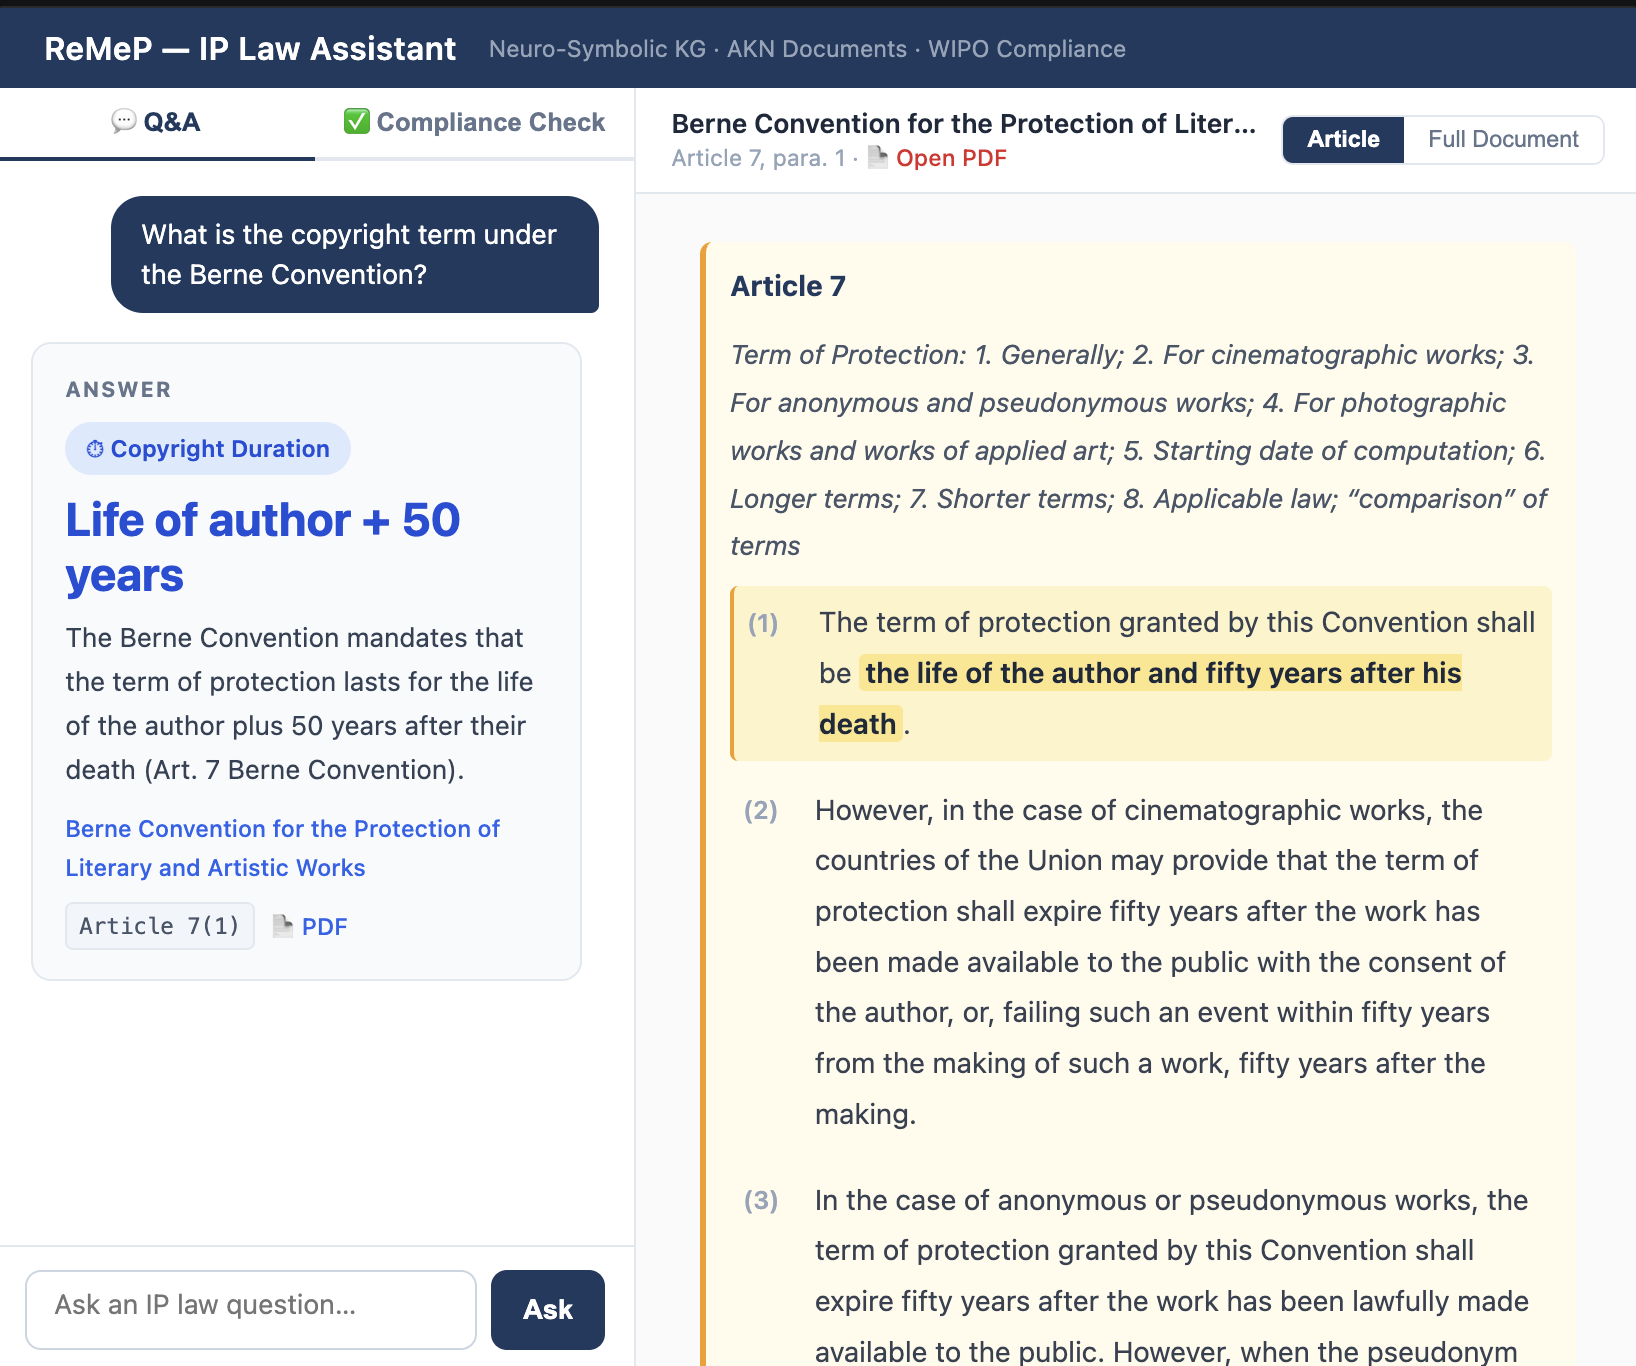
\includegraphics[width=\textwidth]{screenshot_qa.png}
    \caption{Q\&A mode: answer card with citation, AKN article
    rendered with highlighted supporting span, and FRBR meta bar
    (authenticity badge, applicability date, official-source link).}
  \end{subfigure}
  \hfill
  \begin{subfigure}[t]{0.47\textwidth}
    \centering
    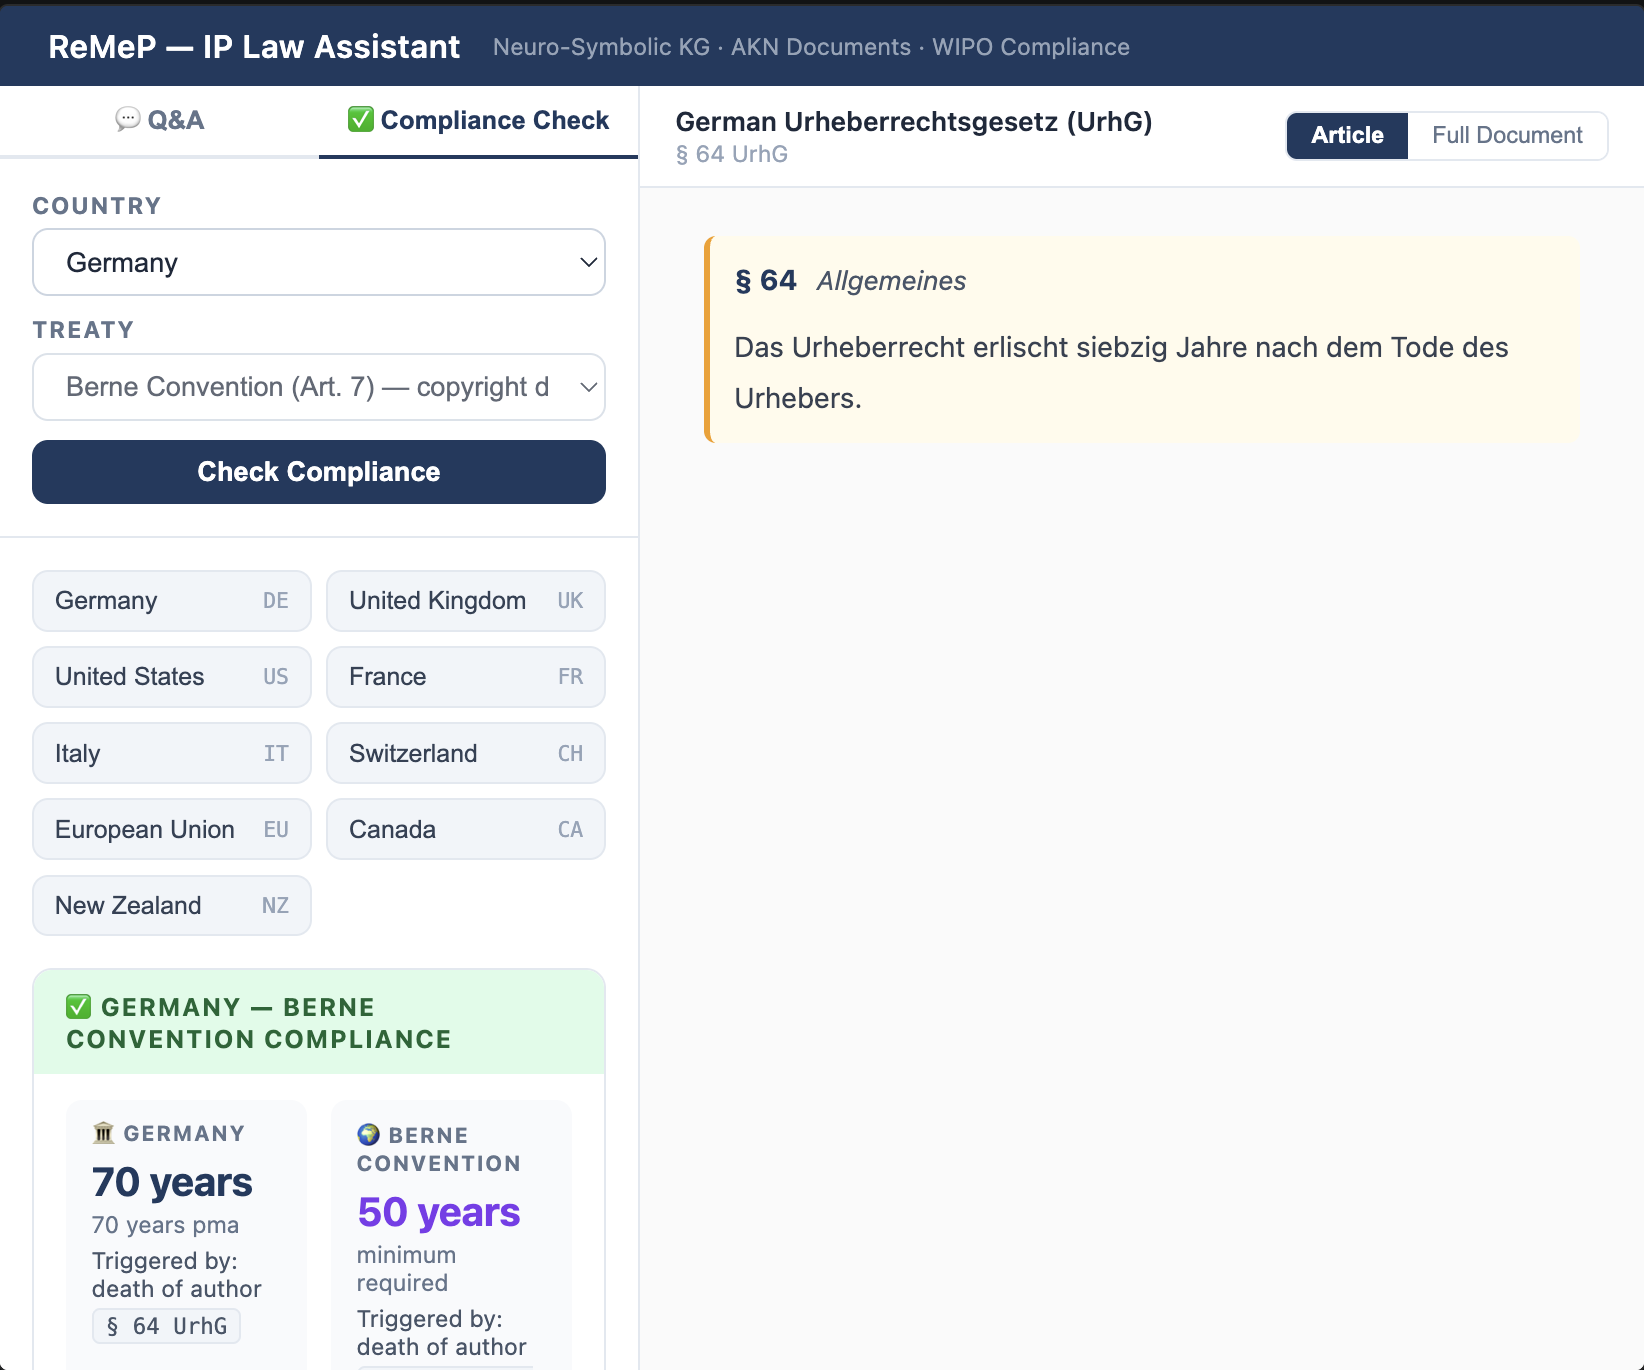
\includegraphics[width=\textwidth]{screenshot_compliance.png}
    \caption{Compliance Check mode: side-by-side comparison of national
    copyright duration vs.\ Berne Convention minimum, with verdict
    and margin in years.}
  \end{subfigure}
  \caption{LEXIA UI in Q\&A and Compliance Check modes.}
  \label{fig:screenshots}
\end{figure}

% ── 5. Evaluation ───────────────────────────────────────────────────────
\section{Evaluation}

\paragraph{Q\&A mode.}
Questions in Italian, English, French, and German are correctly enriched
and routed to the right jurisdiction and rule type. AKN passage extraction
is verified for all nine corpora, covering both \texttt{<article>} and
\texttt{<section>} provision types. Grounded answers always cite the
article reference derived from KG evidence, not from LLM parametric
memory.

\paragraph{Compliance checking.}
All nine jurisdictions yield correct verdicts. Table~\ref{tab:compliance}
shows the results. New Zealand (50~years, exactly at the Berne minimum) is
correctly classified as compliant with zero margin; all 70-year
jurisdictions as compliant $+20$~years above the minimum. The compliance
margin is computed in under 20\,ms with no LLM involvement.

\begin{table}[H]
\centering
\caption{Berne Convention Art.~7 compliance results (9~jurisdictions).}
\label{tab:compliance}
\begin{tabularx}{\textwidth}{lXccc}
\toprule
\textbf{Code} & \textbf{Jurisdiction} &
\textbf{Duration} & \textbf{Margin} & \textbf{Verdict} \\
\midrule
CA & Canada           & 70 years pma & $+$20 & \textcolor{green!60!black}{Compliant} \\
EU & EU Directive     & 70 years pma & $+$20 & \textcolor{green!60!black}{Compliant} \\
FR & France           & 70 years pma & $+$20 & \textcolor{green!60!black}{Compliant} \\
DE & Germany          & 70 years pma & $+$20 & \textcolor{green!60!black}{Compliant} \\
IT & Italy            & 70 years pma & $+$20 & \textcolor{green!60!black}{Compliant} \\
NZ & New Zealand      & 50 years pma & $\pm$0 & \textcolor{green!60!black}{Compliant} \\
CH & Switzerland      & 70 years pma & $+$20 & \textcolor{green!60!black}{Compliant} \\
UK & United Kingdom   & 70 years pma & $+$20 & \textcolor{green!60!black}{Compliant} \\
US & United States    & 70 years pma & $+$20 & \textcolor{green!60!black}{Compliant} \\
\bottomrule
\end{tabularx}
\end{table}

\paragraph{Authentic source attribution.}
FRBR Work URIs are extracted and rendered for all nine corpora.
Authenticity flags vary: UK (\texttt{FRBRprescriptive}), Switzerland and
Italy (\texttt{FRBRauthoritative}), others absent. ELI URIs are present
for Italy and Switzerland.

\paragraph{Point-in-time navigation.}
The date picker correctly resolves Italian copyright law versions across
1941--2025. Selecting 1973-05-30 returns V5 (in force since 1955-01-27);
selecting 1973-06-01 returns V6 (in force since 1973-05-31), demonstrating
day-level precision over the 68-version index.

% ── 6. Limitations ──────────────────────────────────────────────────────
\section{Limitations and Future Work}

\paragraph{Temporal KG triples.}
Point-in-time navigation currently operates at the document level: the
entire AKN expression is swapped. The KG itself carries no
\texttt{valid\_from}/\texttt{valid\_until} timestamps on individual
triples. Adding temporal validity via RDF-star and querying with
SPARQL-star would enable temporally grounded compliance questions such as
``Was France compliant on 1995-01-01?'' entirely at the KG level.

\paragraph{Bidirectional monitoring.}
Only national $\to$ treaty compliance is implemented (does country $X$
meet treaty minimum $Y$?). The reverse direction---which countries have
not yet transposed Directive $X$?---requires transposition deadline data
not present in the current dataset.

\paragraph{Semantic equivalence reasoning.}
Numeric comparison ($70 \geq 50$) handles duration correctly. For
rights-dimension compliance (e.g.,\ ``Does country $X$'s communication
right cover WIPO's \emph{making available}?'') OWL-RL reasoning over the
IPROnto class hierarchy is required.

\paragraph{KG scale and automation.}
The dataset covers 3~rule types $\times$ 9~jurisdictions = 27~core nodes.
A production system requires automatic AKN-to-RDF ingestion covering all
IPROnto dimensions and integration with live sources (EUR-Lex, national
gazette APIs).

\paragraph{eId-based subject URIs.}
Subject URIs follow the pattern \texttt{ex:CH\_duration} rather than
\texttt{ex:CH\_art\_29}. Embedding the \texttt{eId} into the URI would
allow SPARQL queries to directly dereference AKN provisions, eliminating
the ArticleLocator lookup at query time.

\paragraph{Point-in-time coverage.}
The 68-version temporal index covers only Italy (Normattiva corpus). The
same approach is directly applicable to any jurisdiction with versioned
AKN corpora (EUR-Lex, legislation.gov.uk).

% ── 7. Conclusion ───────────────────────────────────────────────────────
\section{Conclusion}

This prototype demonstrates that a neuro-symbolic pipeline---LLM for query
understanding and answer generation, SPARQL+RDF for structured retrieval,
AKN XML for source grounding---is a viable and implementable architecture
for legal IP compliance monitoring within a hackathon timeframe. The two
new components---authentic source attribution via FRBR/ELI extraction, and
point-in-time navigation via the 68-version Italian legislative corpus---
directly address the requirements for traceable, temporally grounded legal
information retrieval. The compliance checker, grounded in integer-typed
KG triples and \texttt{ipronto:compliesWith} links, confirms that the
symbolic layer can answer structured compliance questions without LLM
involvement, reducing both latency and hallucination risk.

The limitations identified in Section~6---temporal KG triples,
bidirectional monitoring, OWL reasoning, KG scale---constitute the roadmap
from this hackathon prototype toward a production-grade bidirectional
monitoring system.

Source code is available at:
\url{https://github.com/Stocastico96/ReMeP_Hackathon_26}

% ── References ──────────────────────────────────────────────────────────
\begin{thebibliography}{99}

\bibitem{palmirani2011}
M.~Palmirani and F.~Vitali.
\newblock Akoma-Ntoso for legal documents.
\newblock In \emph{Legislative XML for the Semantic Web}, pages 75--100.
  Springer, Dordrecht, 2011.
\newblock \url{https://doi.org/10.1007/978-94-007-1887-6_5}

\bibitem{ifla1998}
IFLA Study Group on the Functional Requirements for Bibliographic Records.
\newblock \emph{Functional Requirements for Bibliographic Records (FRBR)}.
\newblock IFLA, M\"{u}nchen, 1998.

\bibitem{eli2012}
Publications Office of the European Union.
\newblock European Legislation Identifier (ELI).
\newblock \emph{Official Journal of the EU}, 2012/C~325/02, 2012.
\newblock \url{https://eur-lex.europa.eu/eli-register/about.html}

\bibitem{delgado2003}
J.~Delgado, I.~Gallego, S.~Llorente, and R.~Garc\'{\i}a.
\newblock {IPROnto}: An ontology for intellectual property rights.
\newblock Distributed Multimedia Applications Group (DMAG), Universitat
  Polit\`{e}cnica de Catalunya, 2003.
\newblock \url{http://dmag.ac.upc.edu/ontologies/ipronto.owl}

\bibitem{palmirani2011lrml}
M.~Palmirani, G.~Governatori, A.~Rotolo, S.~Tabet, H.~Boley, and A.~Paschke.
\newblock {LegalRuleML}: {XML}-based rules and norms.
\newblock In \emph{RuleML 2011}, volume 6826 of \emph{LNCS}, pages 298--312.
  Springer, 2011.

\bibitem{nardi2026}
D.~Nardi et al.
\newblock An analysis of ontologies for the intellectual property domain.
\newblock In \emph{Proceedings of IRIS~2026} (this volume), 2026.

\bibitem{hitzler2022}
P.~Hitzler and M.~K.~Sarker.
\newblock \emph{Neuro-Symbolic Artificial Intelligence: The State of the Art}.
\newblock IOS Press, Amsterdam, 2022.

\bibitem{huang2023}
L.~Huang et al.
\newblock A survey on hallucination in large language models: Principles,
  taxonomy, challenges, and open questions.
\newblock arXiv:2311.05232, 2023.

\bibitem{oasis2018}
OASIS.
\newblock Akoma Ntoso Version 1.0.
\newblock OASIS Standard, 2018.
\newblock \url{http://docs.oasis-open.org/legaldocml/akn-core/v1.0/}

\bibitem{berne1886}
WIPO.
\newblock Berne Convention for the Protection of Literary and Artistic Works,
  Art.~7.
\newblock WIPO, Geneva, 1886 (as amended 1979).
\newblock \url{https://www.wipo.int/treaties/en/ip/berne/}

\end{thebibliography}

\end{document}
